\documentclass[12pt]{article}
\usepackage{graphicx}
\usepackage{hyperref}
\usepackage[top=2.75in, left=1in, right=1in, bottom=0.25in]{geometry}
\usepackage[utf8]{inputenc}
\usepackage[english]{babel}
\usepackage{fancyhdr}
\usepackage[utf8]{inputenc}
\usepackage{listings}
\usepackage{color}
\usepackage[final]{pdfpages}
\usepackage{multirow}
\usepackage{array}

\definecolor{codegreen}{rgb}{0,0.6,0}
\definecolor{codegray}{rgb}{0.5,0.5,0.5}
\definecolor{codepurple}{rgb}{0.58,0,0.82}
\definecolor{backcolour}{rgb}{0.95,0.95,0.92} 
\lstdefinestyle{mystyle}{
    backgroundcolor=\color{backcolour},   
    commentstyle=\color{codegreen},
    keywordstyle=\color{magenta},
    numberstyle=\tiny\color{codegray},
    stringstyle=\color{codepurple},
    basicstyle=\footnotesize,
    breakatwhitespace=false,         
    breaklines=true,                 
    captionpos=b,                    
    keepspaces=true,                 
    numbers=left,                    
    numbersep=5pt,                  
    showspaces=false,                
    showstringspaces=false,
    showtabs=false,                  
    tabsize=2
} 
\lstset{style=mystyle}

\setlength{\parindent}{4em}
\setlength{\parskip}{1em}
\pagestyle{fancy}
\fancyhf{}
\rhead{Assignment 3}
\lhead{Huan Huang}
\renewcommand{\headrulewidth}{0.4pt}
\renewcommand{\footrulewidth}{0.4pt}
\rfoot{Page \thepage}


\begin{document}
\begin{titlepage}
	\begin{center}
	\Huge{Web Science cs532-s16}\\
	[0.25in]
	\textsc{\Large Assignment 3 Report}\\
	\textsc{\normalsize Dr. Michael L. Nelson}\\
	[4.25in]
	\textsc{\normalsize By: Huan Huang}\\
	\large 02/18/2016\\
	
	
	\end{center}
\end{titlepage}
\newpage

\newgeometry{margin=1in}

\section*{Problem 1}
Download the 1000 URIs from assignment \#2.  ``curl", ``wget", or
``lynx" are all good candidate programs to use.  We want just the
raw HTML, not the images, stylesheets, etc.

\noindent
from the command line:

\begin{verbatim}
% curl http://www.cnn.com/ > www.cnn.com

% wget -O www.cnn.com http://www.cnn.com/

% lynx -source http://www.cnn.com/ > www.cnn.com
\end{verbatim}

\noindent
``www.cnn.com" is just an example output file name, keep in mind
that the shell will not like some of the characters that can occur
in URIs (e.g., ``?", ``\&").  You might want to hash the URIs, like:

\begin{verbatim}
% echo -n ``http://www.cs.odu.edu/show_features.shtml?72" | md5
41d5f125d13b4bb554e6e31b6b591eeb
\end{verbatim}

\noindent
(``md5sum" on some machines; note the ``-n" in echo -- this removes
the trailing newline.) 

\noindent
Now use a tool to remove (most) of the HTML markup.  "lynx" will
do a fair job:

\begin{verbatim}
% lynx -dump -force_html www.cnn.com > www.cnn.com.processed
\end{verbatim}

\noindent
Use another (better) tool if you know of one.  Keep both files 
for each URI (i.e., raw HTML and processed). 

\noindent


\subsection*{Answer}
This problem is pretty straight forward. For each of the 1000 links from last assignment, I used curl to get the web page's raw HTML and save them each separately. To get pass the robot blocks on some websites, I used -A ``Mozilla/5.0 (Macintosh; Intel Mac OS X 10.9; rv:44.0)Gecko/20100101 Firefox/44.0" to disguised my program as a browser. I did try to hash the links to use them as file names, but for some reason, md5sum does not work for over 100 links in my list. Therefore, I just name the files with numbers from 1 to 1000. The file names and their links are saved in a file called ``fileNumWithLink.txt" which will be used in problem 2.

\lstinputlisting[language=Python]{rawHTML.py}

\begin{figure}[h]
\centering
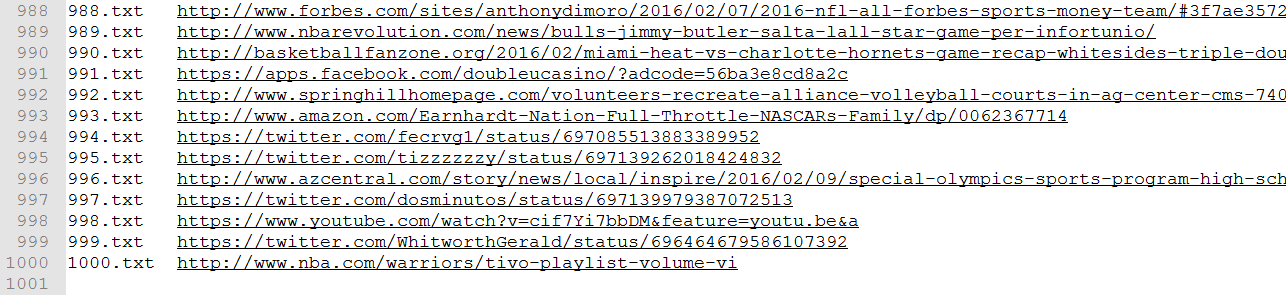
\includegraphics[width=6.5in]{fileNumWithLink.png}
\caption{Sample of part of the fileNumWithLink}
\end{figure}

Next step, for every file of the 1000 raw HTML files, I used lynx to strip away the HTML markups and saved the data into a new file. All of the processed files are named exactly the same from the source files. 

\lstinputlisting[language=Python]{processHTML.py}
\newpage

\begin{figure}[h]
\centering
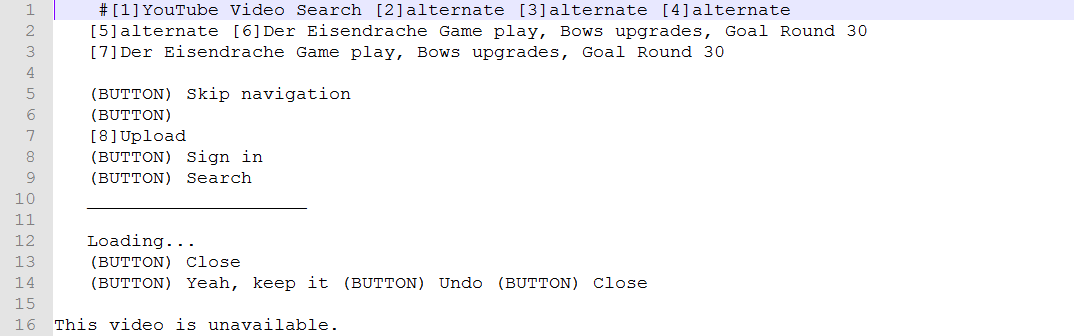
\includegraphics[width=6.5in]{38.png}
\caption{Sample image of a HTML processed file}
\end{figure}

\section*{Problem 2}
Choose a query term (e.g., ``shadow") that is not a stop word
(see week 5 slides) and not HTML markup from step 1 (e.g., ``http")
that matches at least 10 documents (hint: use ``grep" on the processed
files).  If the term is present in more than 10 documents, choose
any 10 from your list.  (If you do not end up with a list of 10
URIs, you've done something wrong).

As per the example in the week 5 slides, compute TFIDF values for
the term in each of the 10 documents and create a table with the
TF, IDF, and TFIDF values, as well as the corresponding URIs.  The
URIs will be ranked in decreasing order by TFIDF values.  For
example:

\noindent
Table 1. 10 Hits for the term ``shadow", ranked by TFIDF.

\noindent
TFIDF	TF	 IDF 	URI\\
0.150	0.014	10.680	http://foo.com/\\
0.044	0.008	 5.510	http://bar.com/

You can use Google or Bing for the DF estimation.  To count the
number of words in the processed document (i.e., the deonminator
for TF), you can use ``wc":

\begin{verbatim}
% wc -w www.cnn.com.processed
   2370 www.cnn.com.processed
\end{verbatim}

It won't be completely accurate, but it will be probably be
consistently inaccurate across all files.  You can use more 
accurate methods if you'd like. Don't forget the log base 2 for IDF, and mind your significant digits!
     
\subsection*{Answer}

For this problem, I wrote a shell script to handle every thing. For every processed file, use wc -w to get the total word count of the file and assign the value into \textit{totalwords}. Use grep -c to find the files contain the word ``gamer'' and count its occurrence in each matching file, then assign the value into \textit{wordmatch}. To get TF, just use \textit{wordmatch} divided by \textit{totalwords}. To get IDF, I searched for the word ``gamer" in Google and received 150000000 matches. Google's estimation of world wide web is roughly 47.1 billion, therefore, IDF is log(47100000000/150000000)/log(2). Lastly, TFIDF is TF multiplied by IDF. I set awk to show 6 digits before and after the dot.

\lstinputlisting[language=Bash]{wordsc.sh}
\newpage

\begin{figure}[h]
\centering
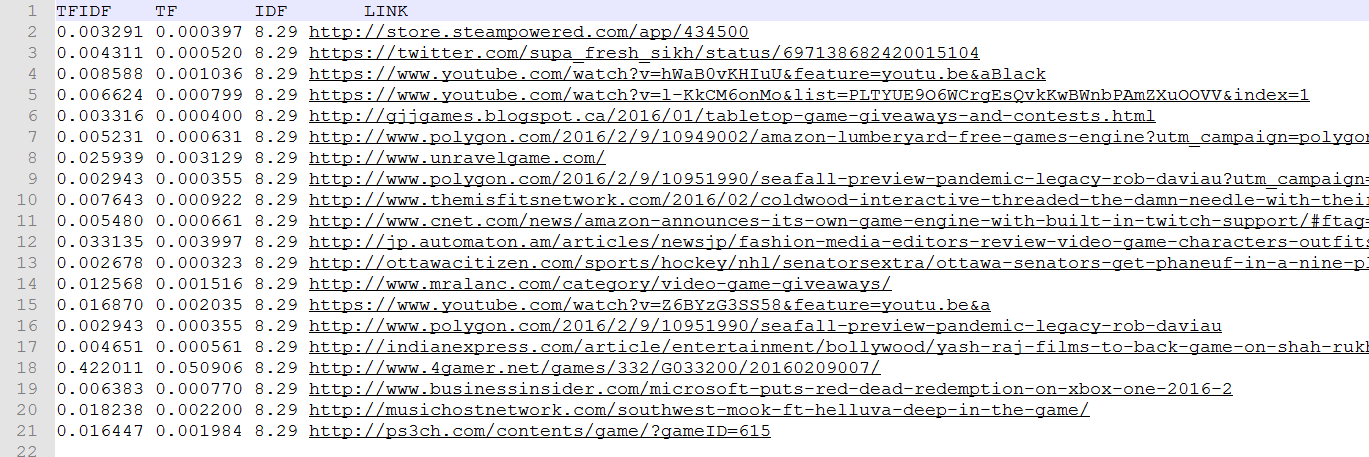
\includegraphics[width=6.5in]{data2.png}
\caption{TFIDF, TF, and IDF for 20 links that match the word ``gamer"}
\end{figure}

\begin{center}
\begin{tabular}{ | m{0.8in} | m{0.8in}| m{0.5in} | m{3.7in} | } 
\hline
TFIDF & TF & IDF & URIs\\
\hline
0.003291 & 0.000397 & 8.29 & http://store.steampowered.com/app/434500 \\ 
\hline
0.004311 & 0.000520 & 8.29 & https://twitter.com/supa\_fresh\_sikh/status/69713868 2420015104 \\ 
\hline
0.008588 & 0.001036 & 8.29 & https://www.youtube.com/watch?v=hWaB0vKHIuU \&feature=youtu.be\&aBlack  \\ 
\hline
0.003316 & 0.000400 & 8.29 & http://gjjgames.blogspot.ca/2016/01/tabletop-game-giveaways-and-contests.html \\ 
\hline
0.005231 & 0.000631 & 8.29 & http://www.polygon.com/2016/2/9/10949002/amaz on-lumberyard-free-games-engine?utm\_campaign=polygon\& utm\_content=chorus\&utm\_medium=social\&utm\_sou rce=twitter \\ 
\hline
0.025939 & 0.003129 & 8.29 & http://www.unravelgame.com/ \\ 
\hline
0.005480 & 0.000661 & 8.29 & http://www.cnet.com/news/amazon-announces-its-own-game-engine-with-built-in-twitch-support/\#ftag=CAD590a51e \\ 
\hline
0.002678 & 0.000323 & 8.29 & http://ottawacitizen.com/sports/hockey/nhl/senator sextra/ottawa-senators-get-phaneuf-in-a-nine-player-deal \\ 
\hline
0.004651 & 0.000561 & 8.29 & http://indianexpress.com/article/entertainment/boll ywood/yash-raj-films-to-back-game-on-shah-rukh-khans-fan/ \\ 
\hline
0.422011 & 0.050906 & 8.29 & http://www.4gamer.net/games/332/G033200/20160 209007/ \\ 
\hline
\end{tabular}
\end{center}

I did use the shell script to pick 10 URIs for me originally, but I encountered a problem with the list in problem 3. Therefore, I changed the script to give me 20 URIs and hand pick 10 URIs from the list.

\newpage

\section*{Problem 3}
Now rank the same 10 URIs from question \#2, but this time 
by their PageRank.  Use any of the free PR estimaters on the web,
such as:

\begin{verbatim}
http://www.prchecker.info/check_page_rank.php
http://www.seocentro.com/tools/search-engines/pagerank.html
http://www.checkpagerank.net/
\end{verbatim}

If you use these tools, you'll have to do so by hand (they have
anti-bot captchas), but there is only 10.  Normalize the values
they give you to be from 0 to 1.0.  Use the same tool on all 10
(again, consistency is more important than accuracy).

\noindent
Create a table similar to Table 1:

\noindent
Table 2.  10 hits for the term "shadow", ranked by PageRank.

\begin{verbatim}
PageRank	 URI
--------	---
0.9       http://bar.com/
0.5       http://foo.com/
\end{verbatim}

\noindent
Briefly compare and contrast the rankings produced in questions 2
and 3.
\newpage

\subsection*{Answer}
To solve this problem, I used the site ``http://www.seocentro.com/tools/search-engines/page rank.html", since it only requires you to fill the captcha once, It made the process a bit faster. However, I encountered the issue of every single one of my URIs have no rank in the page rank check. Therefore, I proceeded by using the hosting site of the URIs. But, because I was only able to use the hosting sites to get the ranks, it is hard to draw conclusions based on the comparison of this ranking and the original TF table in problem 2. Just looking at this ranking table, the result is what I expected. Web sites like Twitter or YouTube which are very well known and aim to server people of any interest would receive the highest ranks. Web sites that are popular amongst people of specific interest would be ranked somewhere in the middle. Then, the random blog pages or new web pages would receive very low rank or no ranking at all.

\begin{table}[h!]
\begin{center}
\begin{tabular}{ | m{0.5in} | m{3in} | } 
\hline
Rank & URIs\\
\hline
1.0 & https://twitter.com \\ 
\hline
0.9 & https://www.youtube.com \\ 
\hline
0.8 & http://www.cnet.com \\ 
\hline
0.7 & http://indianexpress.com \\ 
\hline
0.7 & http://ottawacitizen.com \\ 
\hline
0.6 & http://www.4gamer.net \\ 
\hline
0.6 & http://www.polygon.com \\ 
\hline
0.6 & http://store.steampowered.com \\ 
\hline
0.0 & http://gjjgames.blogspot.ca \\ 
\hline
0.0 & http://www.unravelgame.com \\ 
\hline
\end{tabular}
\end{center}
\caption{A ranking of the 10 URIs from problem2}
\label{Table 2:}
\end{table}

\end{document}